\section{Component-wise SPMD at Macro Scale}
\label{sec:modelling_macro}

We first explore {\em SPMD at macro-scale}, \ie setting one equation
for each interval at the second-scale, \eg between 1 to 5 seconds,
based on two justifications.  First, the power monitor reading
resolution of 0.2ms allows us to have accurate energy (average power
draw) readings at the 1-second granularity. Second, since the GPU
typically goes through the Busy and Idle states at least once in every
16.7ms, using intervals at the second-scale potentially allows us to capture 
diverse GPU and CPU usage, \eg over 
60 or more such rendering intervals, which helps
the regression solver to output meaningful solutions.


\begin{figure*}[tb]
    \centering
    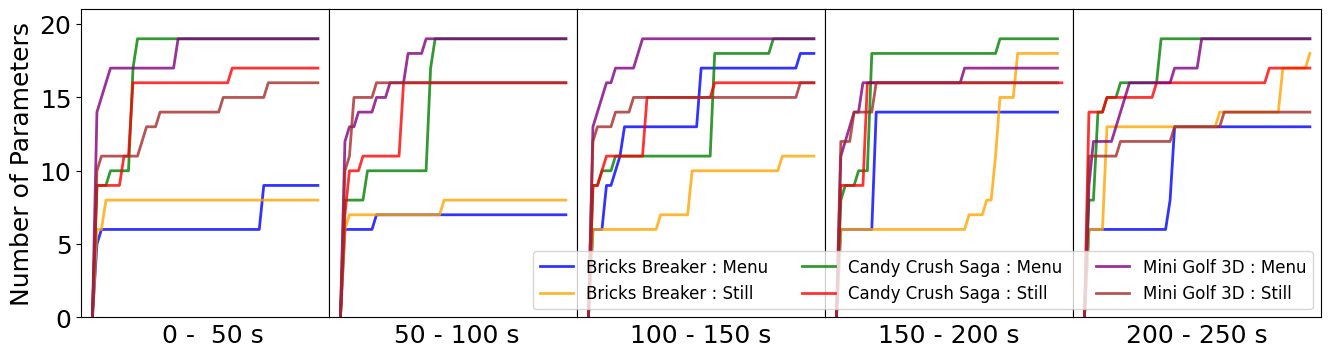
\includegraphics[width=\textwidth]{figures/004_Pixel4_cummulative_parameters.png}
    \vspace{-0.2in}
    \caption{The cumulative number of unique parameters over app run duration in five 50-second segments on Pixel 4.}
    \label{fig:number_parameters_vs_duration_100s}
    \vspace{-0.1in}
\end{figure*}

\paragraph{How Many Systems of Equations?}
\label{subsec:relation}
Since our app run duration are of 250 seconds each, under macro-scale
SPMD, varying per-equation time interval $t_e$ between 1s to 5s gives us
between 50 to 250 equations. To explore how many equations should be
used, we first measure how the number of unique model parameters
varies with the app run duration.

Figure~\ref{fig:number_parameters_vs_duration} shows the cumulative
number of unique power model parameters over a 250-second app run
duration for the six app scenarios on Pixel 4. We make the following
observations.
(1) The number of unique model parameters increases with the app run
duration, with the maximum ranging between 17 (for the Candy Crush Saga Still
scenario) and 19 for (the Mini Golf 3D Menu scenario).
(2) The GPU stayed at one frequency and contributed 2 parameters (Busy
and Idle power in that frequency) for all 6 app scenarios, and the
remaining 15 to 17 parameters are CPU core model parameters.  Similar
trends are observed for the other two phones.

Figure~\ref{fig:number_parameters_vs_duration} does not show the
number of unique model parameters in smaller segments of the app
run.  To see this, we plot in
Figure~\ref{fig:number_parameters_vs_duration_100s} the cumulative
number of unique model parameters over each 50-second time
segment, for the 6 app scenarios.  We see that the curves for all 
five 50-second segments look very similar, suggesting that the apps'
usage of both the CPU and GPU are similar.  However, the total number
of unique model parameters in each of the 50-second segment is
lower when compared with the full 250-second segment. For example, 
with Bricks Breaker Menu, the number of parameters is 18
for the 250-second segment but
reduces to 9, 7, 18, 14 and 13
for the 5 smaller segments.
This suggests that creating a system of equations for a shorter epoch in general may have
fewer unknowns than for a longer epoch.
% \dcomment{'Clarify epoch'}

\if 0
\cut{ 
\begin{figure}[tp]
    \centering
    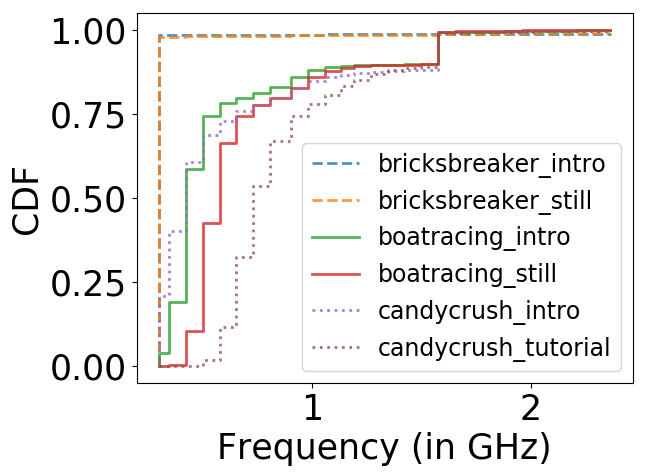
\includegraphics[width=0.65\columnwidth]{figures/cdf_frequency_residence.png}
    \vspace{-0.1in}
    \caption{CDF of the total time spent in each CPU frequencies for 6 app scenarios.}
    \label{fig:cdf_frequency_residence}
    \vspace{-0.1in}
\end{figure}

Finally, to understand how the utilization of different model
parameters vary, we plot in Figure~\ref{fig:cdf_frequency_residence}
the CDF of the percentage of the total time (250 seconds) spent in
each CPU core frequency for the six scenarios. We see the utilizations
are uneven: the top 5 parameters in each app scenario account for
75.20\% to 98.76\% of the total app run duration across the 6 app
scenarios.  In contrast, the utilization of the single GPU frequency
experience in each app scenario varies between 14.72\% and 64.51\%.  
}
\fi



Based on the above exploration, we experimented with 3 alternatives
for creating the system of equations for each app scenario, by varying
the app run duration per system between 50 and 250 seconds, and the
interval per equation between 1 and 5 seconds, while ensuring that
the number of equations per system is 50 or more. 
The 3 configurations have 50 equations of 1 second each,
250 equations of 1 second each, and 50 equation of 5 second each, respectively,
and are denoted as 50x1, 250x1, and 50x5 thereafter.

\begin{table*}[tb]
     \centering
     \begin{subfigure}[b]{0.30\textwidth}
        \centering
        \caption{50 equations with 1 second equation interval}
    	{ \scriptsize
    	\begin{tabular}{ | p{1.8cm} | p{.2cm} | p{.2cm} | p{.2cm} | p{.2cm} | p{.2cm} | p{.2cm} | }
%    	\begin{tabular}{ | l | c | c | c | c | c | c | }
    		\hline
    		     & \multicolumn{6}{ c|}{Error for each App Sc. (\%)}\\
    		\cline{2-7}
                    Model & \rot{B. Menu} & \rot{B. Still} & \rot{C. Menu} & \rot{C. Still} & \rot{M. Menu} & \rot{M. Still}  \\
    		\hline
                Unconst.             & 0.7 & 0.9 & 0.8 & 1.1 & 1.0 & 0.9 \\
                Const.               & 1.2 & 1.1 & 1.2 & 1.6 & 1.4 & 1.3 \\
                Freq. Const.         & 1.2 & 1.1 & 1.6 & 2.1 & 1.9 & 1.8 \\
                Fix. F. Const.       & 1.2 & 1.1 & 1.6 & 2.1 & 1.9 & 1.8 \\
                TPMD                 & 37 & 45 & 17 & 24 & 27 & 9.2 \\
    		\hline
    	\end{tabular}
    	}
    \end{subfigure}
    \hfill
    \begin{subfigure}[b]{0.30\textwidth}
        \centering
        \caption{250 equations with 1 second equation interval}
    	{ \scriptsize
%    	\begin{tabular}{ | p{1.3cm} | p{.2cm} | p{.2cm} | p{.2cm} | p{.2cm} | p{.2cm} | p{.2cm} | }
        \begin{tabular}{ | p{1.8cm} | p{.2cm} | p{.2cm} | p{.2cm} | p{.2cm} | p{.2cm} | p{.2cm} | }
%    	\begin{tabular}{ | l | c | c | c | c | c | c | }
    		\hline
    		     & \multicolumn{6}{ c|}{Error for each App Sc. (\%)}\\
    		\cline{2-7}
                    Model & \rot{B. Menu} & \rot{B. Still} & \rot{C. Menu} & \rot{C. Still} & \rot{M. Menu} & \rot{M. Still}  \\
    		\hline
                Unconst.             & 0.8 & 0.7 & 1.4 & 1.4 & 1.1 & 1.2 \\
                Const.               & 1.0 & 0.8 & 1.3 & 1.5 & 1.2 & 1.3 \\
                Freq. Const.         & 1.0 & 0.9 & 1.4 & 1.8 & 1.3 & 1.4 \\
                Fix. F. Const.       & 1.0 & 0.9 & 1.4 & 1.8 & 1.3 & 1.4 \\
                TPMD                 & 37 & 45 & 17 & 24 & 27 & 8.5 \\
    		\hline
    	\end{tabular}
    	}
    \end{subfigure}
    \hfill
    \begin{subfigure}[b]{0.30\textwidth}
        \centering
        \caption{50 equations with 5 second equation interval}
    	{ \scriptsize
%    	\begin{tabular}{ | p{1.30cm} | p{.2cm} | p{.2cm} | p{.2cm} | p{.2cm} | p{.2cm} | p{.2cm} | }
        \begin{tabular}{ | p{1.8cm} | p{.2cm} | p{.2cm} | p{.2cm} | p{.2cm} | p{.2cm} | p{.2cm} | }
%    	\begin{tabular}{ | l | c | c | c | c | c | c | }
    		\hline
    		     & \multicolumn{6}{ c|}{Error for each App Sc. (\%)}\\
    		\cline{2-7}
                    Model & \rot{B. Menu} & \rot{B. Still} & \rot{C. Menu} & \rot{C. Still} & \rot{M. Menu} & \rot{M. Still}  \\
    		\hline
                Unconst.             & 0.4 & 0.4 & 0.7 & 0.7 & 0.5 & 0.6 \\
                Const.               & 0.6 & 0.4 & 0.8 & 0.9 & 0.6 & 0.8 \\
                Freq. Const.         & 0.7 & 0.5 & 1.0 & 1.2 & 0.9 & 1.1 \\
                Fix. F. Const.       & 0.7 & 0.5 & 1.0 & 1.2 & 0.9 & 1.1 \\
                TPMD                 & 37 & 45 & 17 & 24 & 27 & 8.5 \\
    		\hline
    	\end{tabular}
    	}
    \end{subfigure}
    \caption{Showing error for all app scenarios for 3 ways of creating the system of equations.}
    \label{tab:macro_3_ways_error}
    \vspace{-0.1in}
\end{table*}

\begin{figure*}[tb]
    \centering
    \begin{subfigure}[b]{0.75\textwidth}
         \centering
         
\includegraphics[width=\textwidth]{figures/label_equations.png}
    \end{subfigure}
    \\
    \hfill
    \centering
     \begin{subfigure}[b]{0.32\textwidth}
         \centering
         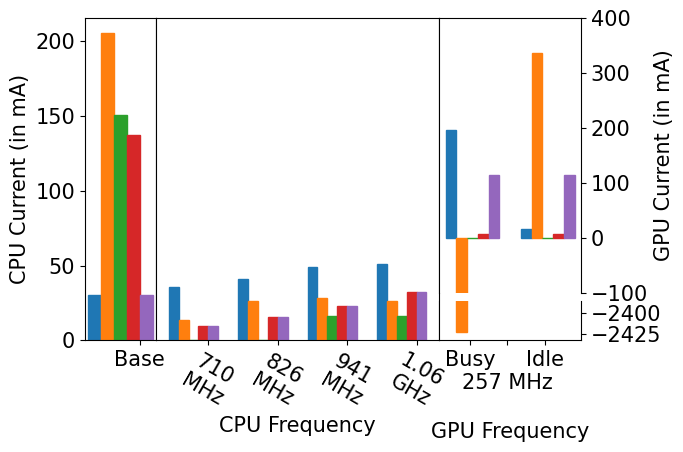
\includegraphics[width=\textwidth]{figures/004_Pixel4_bricksbreaker_menu_50_1_equations.png}
         \caption{50 equations with 1 second equation interval}
         \label{fig:macro_3_ways_50_1}
     \end{subfigure}
    \begin{subfigure}[b]{0.32\textwidth}
         \centering
         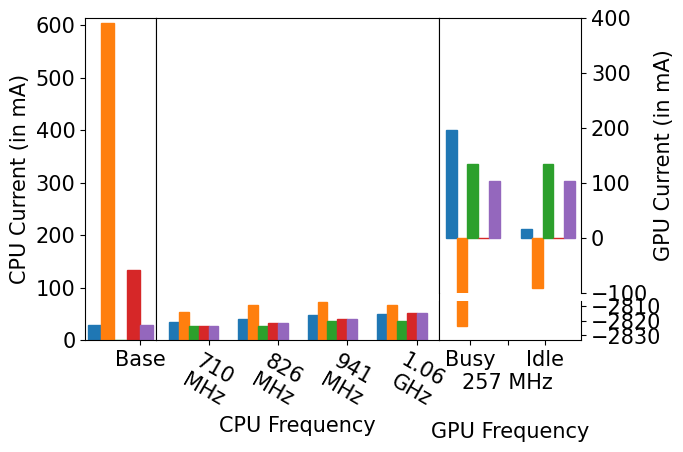
\includegraphics[width=\textwidth]{figures/004_Pixel4_bricksbreaker_menu_250_1_equations.png}
         \caption{250 equations with 1 seconds equation interval}
         \label{fig:macro_3_ways_250_1}
     \end{subfigure}
    \begin{subfigure}[b]{0.32\textwidth}
         \centering
         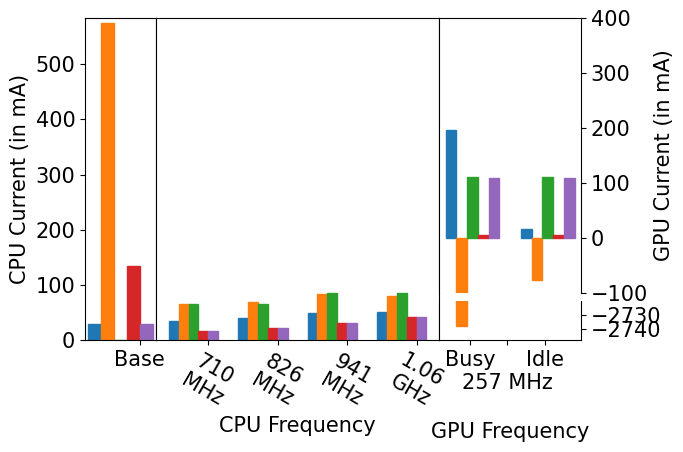
\includegraphics[width=\textwidth]{figures/004_Pixel4_bricksbreaker_menu_250_5_equations.png}
         \caption{50 equations with 5 seconds equation interval}
         \label{fig:macro_3_ways_50_5}
     \end{subfigure}
         \caption{SPMD models for Bricks Breaker Menu scenario on Pixel 4 under
         3 ways of creating the system of equations. 
         (Only model parameters for 4 CPU frequencies with highest utilization are shown due to space constraint.).}
    \label{fig:macro_3_ways}
    \vspace{-0.1in}
\end{figure*}

\paragraph{Detail results on Pixel 4.}
Table~\ref{tab:macro_3_ways_error} summarizes the \comment{mean
  prediction error per equation} of the SPMD models using different
versions of the regression solver for the six app scenarios under the
three ways of creating systems of equations, \comment{on Pixel 4.}
%  \comment{The findings for the other app scenarios and on the other two phones            
% are similar and are omitted due to page limit.}.                                          
We observe that (1) The prediction error only increases slightly as
more constraints are imposed on the regression solver,
\eg from 0.7\%--1.1\% for the unconstrained solver to  1.1\% --1.8\% for
the Fix. Freq. Const version of the solver, for the 50x1 system.
(2) The prediction of SPMD model under the most constrained regression solver,
Fix. Freq. Const, is far lower than that for the TPMD model, \eg ranging
between 9.2\%--45\% for the 50x1 sytem.
(3) The prediction error are consistently low and similar across the
three ways of creating systems of equations, ranging between
1.1\%--1.8\%, 0.9\%--1.8\%, and 0.5\%--1.2\% under the Fix. Freq. Const solver
for the 50x1, 250x1, and 50x5 systems, respectively.

We next look into the actual power model parameters generated by SPMD
for one app scenario in detail.
Figure~\ref{fig:macro_3_ways} shows
the solutions found with these 3 alternative ways of creating systems of
equations for Bricks Breaker Menu scenario on Pixel 4.
For comparison, we include the model parameters derived from
TPMD. We note
that although in general TPMD models are app-agnostic, we listed the
GPU parameters derived for the corresponding app scenarios (as shown
in Figure 1) as the TPMD models here to show how close SPMD-derived
models match the ``carefully'' generated TPMD-derived model.

\st{First, we observed that the ranks of the system of equations is less
than the number of model parameters by more than 1.  The reason is
that the base power shows up in all equations which does not
contribute to the rank.}

\st{As expected, since the systems are under-ranked, the model parameters
output from the unconstrained regression solver look very different
from those found from the TPMD model.}
For the {\it unconstrained solver},
the parameters generated, shown in Figure~\ref{fig:macro_3_ways},
violate some basic properties:
(1) some model parameters generated are negative, \eg the GPU Busy
component power is -2422.15 mA for the 50x1 system  and
is -2737.61 mA for the 50x5 system; and 
%  (2) the CPU power draw at a lower frequency may be higher than the
%  power draw at a higher frequency (for all 3 systems);
(2) The base CPU power for 50x1, 250x1 and 50x5 systems 
is 6.8$\times$, 20.0$\times$, and 19.4$\times$ higher 
than its counterpart in the TPMD model, respectively.
% (3) the GPU Idle power draw generated is higher than the GPU Busy
% power (for all 3 systems). \comment{I do not see that???}

For the {\it constrained solver}, while the parameters generated,
shown as "Constrained" in Figure~\ref{fig:macro_3_ways}, are all
positive and non-decreasing with increasing frequencies, the
CPU power parameters still do not satisfy the monotonicity property;
the parameters for consecutive frequencies often stay the same. 
For example, 
% for the Bricks Breaker Menu scenario,
the CPU power stays at
65.78 mA for 2 of the frequencies from 710 MHz and 825 MHz and again
remains at 86.39 mA for 8 of the frequencies from 941 MHz to 1.80 GHz
for the 50x5 system.

For the {\em Frequency-constrained} solver, the parameters generated, shown in
in Figure~\ref{fig:macro_3_ways}, look very much similar to those in
the TPMD model, but the base power draw ranges between 133.08 mA to
137.11 mA, which is over 4.4$\times$ higher than their counterpart of
30.12 mA observed in the TPMD model for the 3 systems.

{\color{blue}To summarize, by carefully examining the SPMD learning results, we find that }(1) The model parameters differ significantly from
TPMD. For example, for Brick Breakers 50x5 systems, CPU parameters at CPU frequency of
1.61 GHz and 1.92GHz is 133.9 mA and 221.9 mA instead of 85.70 mA and 128.0 mA instead of
TPMD parameters. Also, the power parameters range between
0.28$\times$-1.07$\times$,
0.79$\times$-1.81$\times$,
0.48$\times$-1.86$\times$ their
TPMD counterparts for CPU frequency for the 3 systems.
 %
(2) The GPU Busy and GPU Idle power parameters have the same value in "Fix. F. Const."{\color{blue}--!!!---change this part (tables, figures, values) if you remove Fix. F. Const.---!!!---}
but the counterparts in the TPMD model, the Busy power states is more than 15$\times$
larger than Idle power state.
For example, both parameters are 0.0 mA, 99.1 mA amd 109.2 mA for Bricks Breaker Menu
on all the 3 phones respectively.

\st{To overcome the under-rank problem, we fixed the base power to the
constant value of 30.12 mA as seen in the TPMD model which makes the
rank equal to the number of parameters for the 3 systems. 
With this approach, the parameters generated by the solver, 
shown in the rows labeled "Fix. F. Const.",
only changed slightly;}{\color{blue}---!!!--because we don't need rank, maybe we can remove the Fix. F. Const in the table?--!!!-} 
% the solver split the excessive base power and
% moved them into the GPU Busy and Idle power, and as a result the trend of all the
% parameters now look similar to those observed in the TPMD model.
% \comment{
% However, the generated model parameters still suffer two major problems: 
% (1) The model parameters differ significantly from
% TPMD. For example, for Brick Breakers 50x5 systems, CPU parameters at CPU frequency of
% 1.61 GHz and 1.92GHz is 133.9 mA and 221.9 mA instead of 85.70 mA and 128.0 mA instead of
% TPMD parameters.
% % Similarly, we observe for GPU parameters, Busy and Idle power parameters are both
% % 109.2 mA instead of 196.6 mA and 15.81 mA TPMD parameters.
% Also, the power parameters range between
% 0.28$\times$-1.07$\times$,
% 0.79$\times$-1.81$\times$,
% 0.48$\times$-1.86$\times$ their
% TPMD counterparts for CPU frequency for the 3 systems.
%  %
% (2) The GPU Busy and GPU Idle power parameters have the same value in "Fix. F. Const."{\color{cyan}--!!!---change this part if you remove Fix. F. Const.---!!!---}
% but the counterparts in the TPMD model, the Busy power states is more than 15$\times$
% larger than Idle power state.
% For example, both parameters are 0.0 mA, 99.1 mA amd 109.2 mA for Bricks Breaker Menu
% on all the 3 phones respectively.
% }

{\color{blue}Besides those qualitative evidences that the modeling results of SPMD may be invalid, we also use F-test and $R^2$-measurement to explain the regression solutions for the SPMD modeling results are not valid. --!!-PLEASE FILL RESULTS HERE-!!--}
\dcomment{
We observe that the $R^2$ value varies between 0.05-0.97, 0.24-0.97 and 0.47-0.89 for the
three phones respectively. This shows that for some app scenarios the
curve\_fit fail.
For example, for Candy Crush Still in Pixel 4 the $R^2$ is 0.47.
The inability of able to fit is showed in the average error of
1.2\% which is the highest among of all the app scenarios in Pixel 4.
The minimum singular value is 4.6e-4,
causing the system susceptibility to
$4.6e-4^{-1}$$\approx$$2173\times$ the measurement noise.
% The min singular values fall in the 
The the minimum singular values are between
6.25e-16 - 2.20e-3,
9.65e-19 - 6.12e-3
and
4.58e-20 - 3.67e-3 for the 3 phones respectively.
% The min and max singular values differs by 5.21e+3$\times$-1.01e+6$\times$,
% 2.16e+3$\times$-1.35e+16$\times$ and 1.75e+3$\times$-1.02e+20$\times$ for the 3 phones.
% The large ratio means that the system of equations are very sensitive to any noise.
}

% \paragraph{Results and Validation.}
% Using the 50x5 system of equations, we applied the
% Fix. F. Const. {\color{cyan}!!!--Again, need change if remove Fix. F. Const--!!!} version of SPMD to all 6 app
% scenarios. Figures~\ref{fig:macro_equations}(a)-(c)
% show that SPMD generated models result in much smaller 
% predictor erros for all 6 app scenarios compared to the TPMD generated models.
% However, Figures~\ref{fig:macro_equations}(d)-(f)
% again show that the SPMD-generated model
% parameter suffer the same two problems
% as in the case of the Bricks Breaker Menu scenario, \ie 
% \comment{(1) The model parameters differ significantly from
%   TPMD; (2) The GPU Busy and GPU Idle power parameters are similar
%   which are very different from their counterparts in the TPMD model.}

\begin{figure*}[tb]
     \centering
     \begin{subfigure}[b]{0.32\textwidth}
        \centering
	    \caption{Pixel 2: TPMD vs macro-SPMD error}
	    \vspace{-0.05in}
    	{ \scriptsize
%    	\begin{tabular}{ | p{1.3cm} | p{.2cm} | p{.2cm} | p{.2cm} | p{.2cm} | p{.2cm} | p{.2cm} | }
        \begin{tabular}{ | p{1.8cm} | p{.2cm} | p{.2cm} | p{.2cm} | p{.2cm} | p{.2cm} | p{.2cm} | }
%    	\begin{tabular}{ | l | c | c | c | c | c | c | }
    		\hline
    		     & \multicolumn{6}{ c|}{Error for each App Sc. (\%)}\\
    		\cline{2-7}
                    Model & \rot{B. Menu} & \rot{B. Still} & \rot{C. Menu} & \rot{C. Still} & \rot{M. Menu} & \rot{M. Still}  \\
    		\hline
                Fix. F. Const.       & 0.9 & 1.1 & 1.2 & 0.6 & 0.8 & 0.7 \\
                TPMD                 & 18 & 28 & 13 & 3.4 & 45 & 6.0 \\
    		\hline
    	\end{tabular}
    	}
    	% \vspace{-0.05in}
	    % \caption{Pixel 2: TPMD vs macro-SPMD error}
    \end{subfigure}
    \hfill
    \begin{subfigure}[b]{0.32\textwidth}
        \centering
        \vspace{-0.3in}
	    \caption{Moto Z3: TPMD vs macro-SPMD error}
	    \vspace{-0.05in}
    	{ \scriptsize
%    	\begin{tabular}{ | p{1.3cm} | p{.2cm} | p{.2cm} | p{.2cm} | p{.2cm} | p{.2cm} | p{.2cm} | }
        \begin{tabular}{ | p{1.8cm} | p{.2cm} | p{.2cm} | p{.2cm} | p{.2cm} | p{.2cm} | p{.2cm} | }
%    	\begin{tabular}{ | l | c | c | c | c | c | c | }
    		\hline
    		     & \multicolumn{6}{ c|}{Error for each App Sc. (\%)}\\
    		\cline{2-7}
                    Model & \rot{B. Menu} & \rot{B. Still} & \rot{C. Menu} & \rot{C. Still} & \rot{M. Menu} & \rot{M. Still}  \\
    		\hline
                Fix. F. Const.       & 1.8 & 0.3 & 2.6 & 0.4 & 0.2 & 26 \\
                TPMD                 & 39 & 11 & 31 & 19 & 5.9 & 39 \\
    		\hline
    	\end{tabular}
    	}
    	% \vspace{-0.05in}
	    % \caption{Moto Z3: TPMD vs macro-SPMD error}
    \end{subfigure}
    \hfill
    \begin{subfigure}[b]{0.32\textwidth}
        \centering
	    \caption{Pixel 4: TPMD vs macro-SPMD error}
	    \vspace{-0.05in}
    	{ \scriptsize
%    	\begin{tabular}{ | p{1.3cm} | p{.2cm} | p{.2cm} | p{.2cm} | p{.2cm} | p{.2cm} | p{.2cm} | }
        \begin{tabular}{ | p{1.8cm} | p{.2cm} | p{.2cm} | p{.2cm} | p{.2cm} | p{.2cm} | p{.2cm} | }
%    	\begin{tabular}{ | l | c | c | c | c | c | c | }
    		\hline
    		     & \multicolumn{6}{ c|}{Error for each App Sc. (\%)}\\
    		\cline{2-7}
                    Model & \rot{B. Menu} & \rot{B. Still} & \rot{C. Menu} & \rot{C. Still} & \rot{M. Menu} & \rot{M. Still}  \\
    		\hline
                Fix. F. Const.       & 0.7 & 0.5 & 1.0 & 1.2 & 0.9 & 1.1 \\
                TPMD                 & 37 & 45 & 17 & 24 & 27 & 8.5 \\
    		\hline
    	\end{tabular}
    	}
    	% \vspace{-0.05in}
	    % \caption{Pixel 4: TPMD vs macro-SPMD error}
    \end{subfigure}
    \\
         \vspace{+0.1in}
         \centering
     \begin{subfigure}[b]{\textwidth}
         \centering
         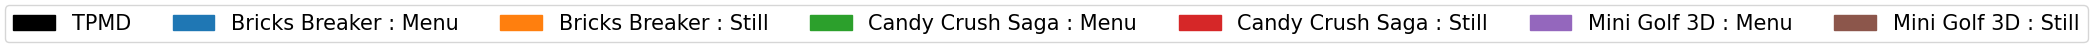
\includegraphics[width=\textwidth]{figures/label_macro_equations.png}
    \end{subfigure}
    \\
    \hfill
    \centering
     \begin{subfigure}[b]{0.32\textwidth}
         \centering
         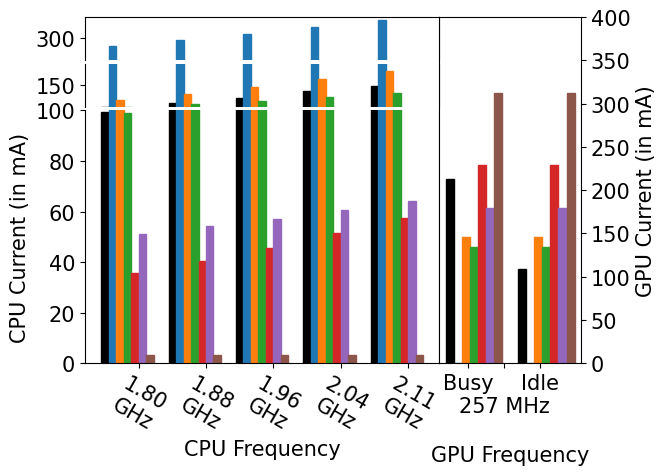
\includegraphics[width=\textwidth]{figures/002_Pixel2_250_5_macro_equations.png}
         \label{fig:macro_equations_p2}
         \vspace{-0.25in}
         \caption{Pixel 2: TPMD vs macro-SPMD coefficients}
     \end{subfigure}
    \begin{subfigure}[b]{0.32\textwidth}
         \centering
         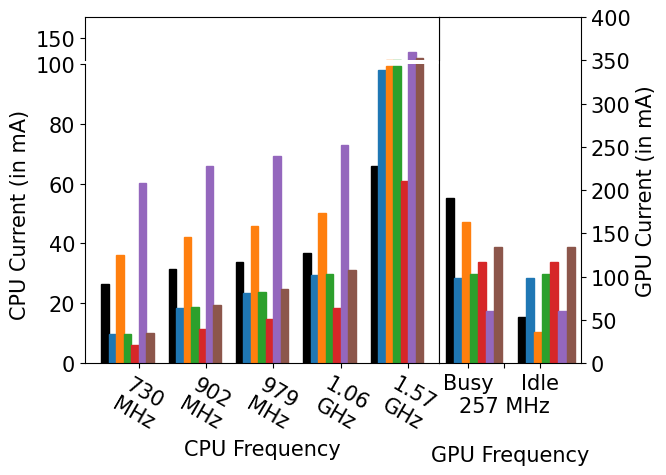
\includegraphics[width=\textwidth]{figures/003_MotoZ3_250_5_macro_equations.png}
         \label{fig:macro_equations_z3}
         \vspace{-0.25in}
         \caption{Moto Z3: TPMD vs macro-SPMD coefficients}
     \end{subfigure}
    \begin{subfigure}[b]{0.32\textwidth}
         \centering
         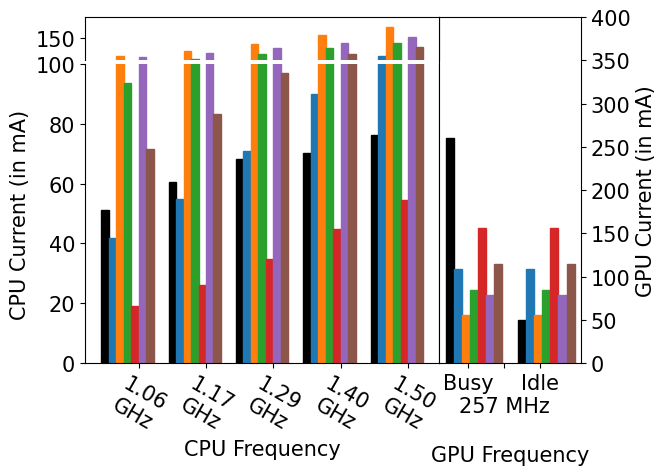
\includegraphics[width=\textwidth]{figures/004_Pixel4_250_5_macro_equations.png}
         \label{fig:macro_equations_p4}
         \vspace{-0.25in}
         \caption{Pixel 4: TPMD vs macro-SPMD coefficients}
     \end{subfigure}

    \caption{Model parameters derived by macro-scale SPMD for 50x5 system on the
        3 phones. TPMD for GPU are from Figure~\ref{fig:gpu_model}.
        (Only model parameters for 5 CPU frequencies with highest utilization are
        shown due to space constraint.) (The GPU parameter for TPMD
        is represented by average over all app scenarios GPU parameters.)}
    \label{fig:macro_equations}
   % \vspace{-0.1in}
\end{figure*}

\paragraph{Analysis.}
{\color{blue}We dig deeper into one the those experiments to \ie 50x5, to
understand why SPMD solutions are invalid. As shown in Table~\ref{tab:macro_rank_singular}, we find that the smallest singular value of the design matrix of the linear regression is close to zero. As we stated in the footnote of Page~3, this implies that the linear regression result will be very sensitive to even a small amount of noise. Roughly speaking, when equations are similar to each other, the smallest singular value of the design matrix is usually close to zero. }

% We dig deeper into one of the the full-rank system, \ie 50x5, to
% understand why SPMD generates very different parameters compared to
% TPMD.
% Since the rank of the system is already
%   full, we calculated the singular values for these equations.
%   Table~\ref{tab:macro_rank_singular} shows that each of the system
%   of equations has only 1 dominating singular value, suggesting that
%   the matrix (formed by coefficients of unknown variables in the
%   tight-hand-side (RHD) of those equations) has only one dominating
%   direction. This indicates that all the equations are basically
%   describing the same state of power usage, and thus lacks diversity.


% \begin{table*}[tb]
% \centering
% {\small
%     \caption{The rank and singular values for the set of equations for macro-scale "F. Freq. Const. SPMD" for 50x5 system on Pixel 4. (Top 11 singular values are shown.)\comment{Will reduce number of singular values later.}}
%     \vspace{-0.1in}
%     \begin{tabular}{|c|c|c|c|c|c|c|c|c|c|c|c|c|c|c|c|c|}
%     \hline
%         App & Scenario & \# of Eqns. & \# of Vars. &  \multicolumn{11}{c|}{Singular Values} & $R^{2}$ & F-Test \\
%         \hline
%          \multirow{2}{15mm}{Bricks Breaker} & Menu & 50 & 18 & 6.54  & 0.37  & 0.17  & 0.10  & 0.04  & 0.02  & 0.02  & 0.01  & 0.01  & 0.00  & 0.00 & 0.68 & \\
%          \cline{2-17}
%          & Still &  50 & 19 & 6.73  & 0.38  & 0.34  & 0.16  & 0.03  & 0.02  & 0.02  & 0.01  & 0.01  & 0.01  & 0.00 & 0.83 & \\
%          \hline
%         \multirow{2}{15mm}{Candy Crush Saga} & Menu &  50 & 19 & 6.79  & 0.49  & 0.19  & 0.10  & 0.08  & 0.03  & 0.03  & 0.02  & 0.02  & 0.01  & 0.01 & 0.73 & \\
%          \cline{2-17}
%          & Still & 50 & 17 & 6.81  & 0.52  & 0.21  & 0.10  & 0.05  & 0.05  & 0.03  & 0.02  & 0.01  & 0.01  & 0.01 & 0.47 & \\
%          \hline
%         \multirow{2}{15mm}{Mini Golf 3D} & Menu & 50 & 19 & 6.41  & 1.62  & 0.47  & 0.38  & 0.18  & 0.06  & 0.03  & 0.02  & 0.02  & 0.01  & 0.01 & 0.80 & \\
%         \cline{2-17}
% 	     & Still & 50 & 17 & 6.46  & 0.99  & 0.34  & 0.19  & 0.11  & 0.06  & 0.04  & 0.03  & 0.02  & 0.01  & 0.01 & 0.89 & \\
% 	     \hline
%     \end{tabular}
%     \label{tab:macro_rank_singular}
%     \vspace{-0.1in}
% }
% \end{table*}
\begin{table*}[tb]
\centering
{\small
    \caption{The {\color{blue}smallest }singular values for the \st{set of equations}{\color{blue}design matrix} for macro-scale "F. Freq. Const. SPMD" for 50x5 system on Pixel 4. (Smallest 11 singular values are shown.)\comment{Will reduce number of singular values later.}}
    \vspace{-0.1in}
    \begin{tabular}{|c|c|c|c|c|c|c|c|c|c|c|c|c|c|c|c|c|}
    \hline
        App & Scenario & \# of Eqns. & \# of Vars. &  \multicolumn{11}{c|}{Smallest  Singular Values} & $R^{2}$ \\
        \hline
         \multirow{2}{15mm}{Bricks Breaker} & Menu & 50 & 18 & 0.01  & 0.01  & 0.00  & 0.00  & 0.00  & 0.00  & 0.00  & 0.00  & 0.00  & 0.00  & 0.00 & 0.68 \\
         \cline{2-16}
         & Still &  50 & 19 & 0.01  & 0.01  & 0.00  & 0.00  & 0.00  & 0.00  & 0.00  & 0.00  & 0.00  & 0.00  & 0.00 & 0.83 \\
         \hline
        \multirow{2}{15mm}{Candy Crush Saga} & Menu &  50 & 19  & 0.02  & 0.01  & 0.01  & 0.01  & 0.01  & 0.01  & 0.00  & 0.00  & 0.00  & 0.00  & 0.00 & 0.73 \\
         \cline{2-16}
         & Still & 50 & 17  & 0.03  & 0.02  & 0.01  & 0.01  & 0.01  & 0.01  & 0.01  & 0.01  & 0.01  & 0.00  & 0.00 & 0.47 \\
         \hline
        \multirow{2}{15mm}{Mini Golf 3D} & Menu & 50 & 19  & 0.02  & 0.01  & 0.01  & 0.01  & 0.01  & 0.01  & 0.01  & 0.01  & 0.00  & 0.00  & 0.00 & 0.80 \\
        \cline{2-16}
	     & Still & 50 & 17  & 0.03  & 0.02  & 0.02  & 0.01  & 0.01  & 0.01  & 0.00  & 0.00  & 0.00  & 0.00  & 0.00 & 0.89 \\
	     \hline
    \end{tabular}
    \label{tab:macro_rank_singular}
    \vspace{-0.1in}
}
\end{table*}
% In addition to lack of diversity in phone component usage which contributed 
% to the sparse singular values, we found that the energy values in LHS of
% the equation   appear to contain  measurement noise which further prevents
% the regression solver from generating meaningful solutions. To see this,
% we plot the distribution of the LHS energy values of the  equations in the
% two systems 250x1 and 50x5, Figures~\ref{fig:y_distribution}(a)-(b) show the
% energy values for the two systems are clustered in a Gaussian distribution
% with standard deviation of 3.04 mA and 5.72 mA, each of which is less than
% 2.45\% compared with the mean value. This Gaussian-like distribution suggests
% that the LHS values of the equations contain measurement noise.
% \comment{PZ: this is not obvious????}

% \begin{figure}[tb]
%     \vspace{-0.1in}
%     \centering
%          \begin{subfigure}[b]{0.49\columnwidth}
%          \centering
%          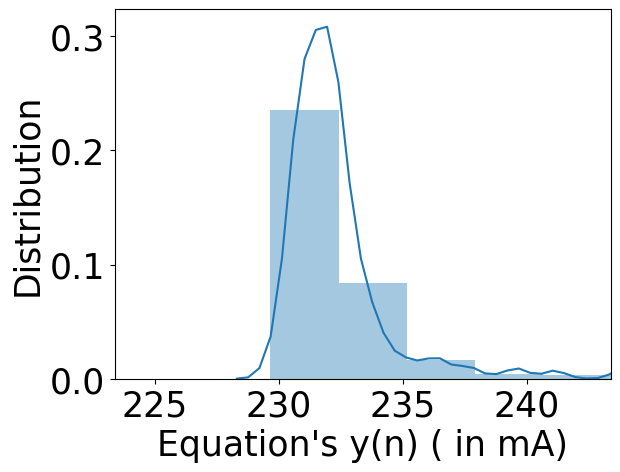
\includegraphics[width=\textwidth]{figures/004_Pixel4_bricksbreaker_menu_250_1_distribution_y_n.png}
%          \caption{250 1-second equations}
%     \end{subfigure}
%     \hfill
%     \begin{subfigure}[b]{0.49\columnwidth}
%          \centering
%          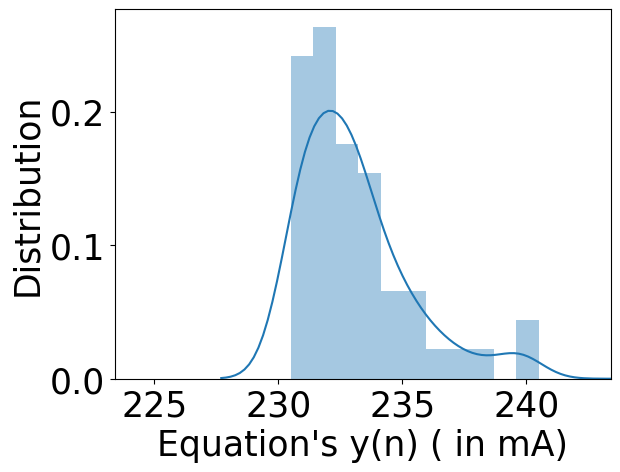
\includegraphics[width=\textwidth]{figures/004_Pixel4_bricksbreaker_menu_250_5_distribution_y_n.png}
%          \caption{50 5-second equations}
%     \end{subfigure}
%     \vspace{-0.1in}
%     \caption{Distribution of the energy terms of the
%     equations for Bricks Breaker Menu scenarios on Pixel 4.}
%     \label{fig:y_distribution}
%     \vspace{-0.2in}
% \end{figure}

\st{To understand why the system of model equations for the 6 app scenarios lack
diversity}{\color{blue}To illustrate the similarity among equations of 1-second interval}, we zoom into the power monitor readings.
Figure~\ref{fig:power_trace_candycrush_menu} shows a snippet of the power monitor
readings during the Candy Crush Saga Menu scenario. We see that the power draw
shows a clear repeating pattern at every 16.7ms interval. This happens due to
typical game app behavior -- a game app typically renders 60 FPS and the graphic
contents rendered within each game scenario are largely similar. As a result,
aggregating the power activities within each of the 1-second interval into one
model equation will result in the set of equations (for the same app scenario)
looking largely similar.

{\color{blue}To summarize, due to the lack of variation of CPU/GPU utilization level in the second-scale, the linear regression used for SPMD becomes very sensitive to the noise and consequently make the modeling results invalid.}

% \comment{To summarize, our experimental results and analysis above suggest that
% the equations created from macro-scale SPMD do not exhibit enough
% diversity and as a result the regression solver even after careful
% adjustments can not output meaningful solutions for the model
% parameters.
% ???
% }
